\LARGE{ \textbf {Лекция №13}}\\
\Large{ \textbf {Демультиплексор.}}\\
DMX\\
Выполняет функцию обратную функции мультиплексирования.
Имеет один вход в общем случае $n$ адресных входов и , если полный то $2^n$ выходов.
Обеспечивает коммутацию сигнала со входа на выход номер которого является десятичным эквивалентом адресного кода.
Демультиплексоров не существует в природе, вместо них используются дешифраторы.

\Large{ \textbf {Сумматоры}}\\
Десумматоров не бывает.\\
SUM - SM\\
Сумматор - узел предназначенный для операции микросложения слов.

В зависмомти от систем счисления различают
\begin{enumerate}
  \item Двоичные
  \item Двоично-десятичные
  \item Прочие
\end{enumerate}

По типу схемы:

\begin{enumerate}
  \item Комбинационные - то есть $ C = A + B $
  \item Накапливающие $ C = A + C $ содержат регистр, в который в начале заносится одно из слагаемых- в данном случае С. Затем складываются.
\end{enumerate}

По разрядеости.
\begin{enumerate}
  \item Одноразряжные
  \item Многоразрядные сумматоры
\end{enumerate}
Для того, чтобы сложить 2 числа, $a,b$ нужно:\\
Сложить их по модулю 2. Должны учесть перенос. Проссумировать по модулю 2 с этим переносом.\\

$CR_i = a_i b_i  a_i CR_{i-1} +a_i CR_{i-1} ==$\\
$a_i b_i + CR_i (a_i +m2+ b_i)$\\
Это полный сумматор, потому что есть прием переноса из предыдущего разряда.\\
Если в сумматоре отсутсвет вход $ CR_i $, то это не полный.\\
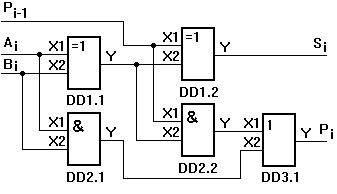
\includegraphics{52}\\


Многоразрядные сумматоры делятся на
\begin{enumerate}
  \item Последовательные - носят теоретический характер.
  Последовательное суммирование выполняется на однорозрядном сумматоре поочередно, разряд за разрядом.
  \item Паралелльные - слагаемые обрабатываются одновременно по всем разрядам.
\end{enumerate}

По способу организации межразрядных переносов паралельные сумматоры разделяют на
\begin{enumerate}
  \item Последовательным переносом
  \item Паралелльным
  \item Групповым переносом
\end{enumerate}

\newpage
\Large{ \textbf {Паралелльные многоразрядные сумматоры}}\\
Сумматоры с последовательным переносом.\\
Схема сумматора с последовательным переносом.\\
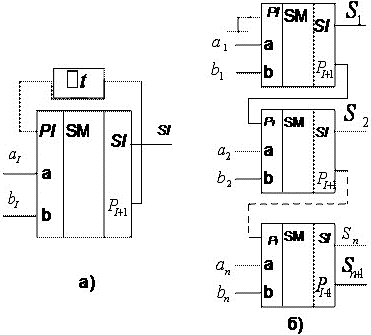
\includegraphics{53}\\
Слагаемые принимаются паралельно, после этого образуются предварительные разрядные суммые, а после появления и распространения  переносов суммы преобретают окончательные значения.
Быстродействие определятся так $ t_{zadsr} = t_{zd.CR} + (n-2) t_{pCR} + t_{pS}  $\\
Первое - время выработки сигнала на первом разряде.\\
Второе слагаемое - время распространения переноса через один разряд.\\
Третье - время выработки суммы в старшем разряде.\\
Достоинство схеммы - простотра и однотипоность разрядов.\\
Недостаток - быстрота. С ростом числа разрядов скорость работы уменьшается. Поэтому на практике используются для максимум 8 разрядов.\\
Для повышения быстродействия сумматоров используются ускоренные способы формирования переноса.\\

\newpage
\textbf{Сумматоры с ускоренным переносом.}\\
$ CR_{n+1} = a_n b_n + (a_n +m2+ b_n) \cdot CR_n $\\
$CR_2 = a_1 b_1 + (a_1 +m2+ b_1) \cdot CR_1 $\\
$CR_3 = a_2 b_2 + (a_2 +m2+ b_2) \cdot CR_2 $\\
Отсюда видно, что значение переноса в каждом разряде можно определить по слагаемым и переносу только в первый разряд.
Перенос в итый разряд реализуется на элементах И, ИЛИ, ИСКЛЮЧАЮЩЕЕ-ИЛИ.
Схема вырабатывающая сигналы переноса так образом, называют схемами ускоренного переноса - CRU.
В этих схемах используются функции генерации переноса - CRG. Функция распространения переноса - CRP.\\
Перенос из итого разряда:\\
$CR_i = a_i b_i  a_i CR_{i-1} +a_i CR_{i-1} ==$\\
$a_i b_i + CR_i (a_i +m2+ b_i)$\\
$a_i b_i = CRG_i$.\\
$ (a_i +m2+ b_i) - CRP_i$.\\
Объеденение схем сумматоров со схемами ускоренного переноса позволяет строить паралельные сумматоры с паралельныи переносом.\\
Длительность переноса в таком случае не зависит от разрядности слагаемых.\\
